%%%%%%%%%%%%%%%%%%%%%%%%%%%%%%%%%%%%%%%%%%%%%%%%%%%%%%%%%%
%   Vorlage von:
%
%   Prof. Dr. Bernhard Drabant
%   Prof. Dr. Dennis Pfisterer
%   Prof. Dr. Julian Reichwald
%
%%%%%%%%%%%%%%%%%%%%%%%%%%%%%%%%%%%%%%%%%%%%%%%%%%%%%%%%%%

%%%%%%%%%%%%%%%%%%%%%%%%%%%%%%%%%%%%%%%%%%%%%%%%%%%%%%%%%%
%	ANLEITUNG: 
%
%   1. Ersetzen Sie firmenlogo.jpg im Verzeichnis img
%   2. Passen Sie alle Stellen im Dokument an, die mit 
%      @stud markiert sind
%
%%%%%%%%%%%%%%%%%%%%%%%%%%%%%%%%%%%%%%%%%%%%%%%%%%%%%%%%%%

%%%%%%%%%%%%%%%%%%%%%%%%%%%%%%%%%%%%%%%%%%%%%%%%%%%%%%%%%%
%	ACHTUNG: 
%
%   Für das Erstellen des Literaturverzeichnisses wird das 
%   modernere Paket biblatex in Kombination mit biber 
%   verwendet -- nicht mehr das ältere BibTex!
%   Bitte stellen Sie ggf. Ihre TeX-Umgebung entsprechend 
%   ein (z.B. TeXStudio: Einstellungen --> Erzeugen --> 
%   Standard Bibliographieprogramm: biber)
%
%%%%%%%%%%%%%%%%%%%%%%%%%%%%%%%%%%%%%%%%%%%%%%%%%%%%%%%%%%

\documentclass[12pt,BCOR=5mm,DIV=12,headinclude=on,footinclude=off,parskip=half,bibliography=totoc,listof=entryprefix,
               toc=listof,pointlessnumbers,plainfootsepline]{scrreprt}

% Elementare Konfigurationen und Definitionen werden geladen
% !TEX root =  master.tex
%      HYPERREF

%%%%%%%%%%%%%%%%%%%%%%%%%%%%%%%%%%%%%%%%%%%%%%%%%%%%%%%%%%
%	ANLEITUNG: 
%
% Passen Sie alle Stellen im Dokument an, die mit 
% @stud markiert sind
%
%%%%%%%%%%%%%%%%%%%%%%%%%%%%%%%%%%%%%%%%%%%%%%%%%%%%%%%%%%

\usepackage{makeidx}         % allows index generation
\usepackage{listings}	%Format Listings properly
\usepackage{lipsum}    %Blindtext
\usepackage{graphicx} % use various graphics formats
\usepackage[german]{varioref} 	% nicer references \vref
\usepackage{caption}	%better Captions
\usepackage{booktabs} %nicer Tabs
\usepackage{array}
\usepackage{chngcntr}
\usepackage[hidelinks=true]{hyperref} % keine roten Markierungen bei Links
\usepackage{fnpct} % Correct superscripts 
\usepackage[T1]{fontenc}
\usepackage[utf8]{inputenc}
\usepackage{calc} % Used for extra space below footsepline
\usepackage{acronym}
\usepackage{algorithm}
\usepackage{algpseudocode}

%
% @stud
%
%	FONT SELECTION: Entweder 1) Latin Modern oder 2) Times / Helvetica
\usepackage{lmodern}             % 1) Latin modern font
%\usepackage{mathptmx}           % 2) Helvetica / Times New Roman fonts (2 lines)
%\usepackage[scaled=.92]{helvet} % 2) Helvetica / Times New Roman fonts (2 lines)

%
% @stud
%
%	LANGUAGE SETTINGS
\usepackage[ngerman]{babel} 	        % german language
\usepackage[german=quotes]{csquotes} 	% correct quoting using \enquote{}
%\usepackage[english]{babel}          % english language
%\usepackage{csquotes} 	              % correct quoting using \enquote{}

%
% @stud
%
% Uncomment the following lines to support hard URL breaks in bibliography 
%\apptocmd{\UrlBreaks}{\do\f\do\m}{}{}
%\setcounter{biburllcpenalty}{9000}% Kleinbuchstaben
%\setcounter{biburlucpenalty}{9000}% Großbuchstaben

%
% @stud
%
%	FOOTNOTES: Count footnotes over chapters
%1 \counterwithout{footnote}{chapter}

%	ACRONYMS
\makeatletter
\@ifpackagelater{acronym}{2015/03/20}
{\renewcommand*{\aclabelfont}[1]{\textbf{{\acsfont{#1}}}}}{}
\makeatother

%	LISTINGS
\renewcommand{\lstlistingname}{Quelltext} 
\renewcommand{\lstlistlistingname}{Quelltextverzeichnis}
\lstset{numbers=left,
	numberstyle=\tiny,
	captionpos=b,
	basicstyle=\ttfamily\small}



%		PAGE HEADER / FOOTER
%	    Warning: There are some redefinitions throughout the master.tex-file!  DON'T CHANGE THESE REDEFINITIONS!
\RequirePackage[automark,headsepline,footsepline]{scrpage2}
\pagestyle{scrheadings}
%\renewcommand*{\pnumfont}{\upshape\sffamily}
%\renewcommand*{\headfont}{\upshape\sffamily}
%\renewcommand*{\footfont}{\upshape\sffamily}
\renewcommand{\chaptermarkformat}{}
\RedeclareSectionCommand[beforeskip=0pt]{chapter}
\clearscrheadfoot

\ifoot[\rule{0pt}{\ht\strutbox+\dp\strutbox}HTW Berlin]{\rule{0pt}{\ht\strutbox+\dp\strutbox}HTW Berlin}
\ofoot[\rule{0pt}{\ht\strutbox+\dp\strutbox}\pagemark]{\rule{0pt}{\ht\strutbox+\dp\strutbox}\pagemark}
\ohead{\headmark}

\newcommand{\TitelDerArbeit}[1]{\def\DerTitelDerArbeit{#1}\hypersetup{pdftitle={#1}}}
\newcommand{\AutorDerArbeit}[1]{\def\DerAutorDerArbeit{#1}\hypersetup{pdfauthor={#1}}}
\newcommand{\Firma}[1]{\def\DerNameDerFirma{#1}}
\newcommand{\Kurs}[1]{\def\DieKursbezeichnung{#1}}
\newcommand{\Abteilung}[1]{\def\DerNameDerAbteilung{#1}}
\newcommand{\Studiengangsleiter}[1]{\def\DerStudiengangsleiter{#1}}
\newcommand{\WissBetreuer}[1]{\def\DerWissBetreuer{#1}}
\newcommand{\FirmenBetreuer}[1]{\def\DerFirmenBetreuer{#1}}
\newcommand{\Bearbeitungszeitraum}[1]{\def\DerBearbeitungszeitraum{#1}}
\newcommand{\Abgabedatum}[1]{\def\DasAbgabedatum{#1}}
\newcommand{\Matrikelnummer}[1]{\def\DieMatrikelnummer{#1}}
\newcommand{\Studienrichtung}[1]{\def\DieStudienrichtung{#1}}
\newcommand{\ArtDerArbeit}[1]{\def\DieArtDerArbeit{#1}}
\newcommand{\Literaturverzeichnis}{Literaturverzeichnis}

\newcommand{\settingBibFootnoteCite}{
	\setlength{\bibparsep}{\parskip}		  % Add some space between biblatex entries in the bibliography
	\addbibresource{bibliography.bib}	    % Add file bibliography.bib as biblatex resource
	\DefineBibliographyStrings{ngerman}{andothers = {{et\,al\adddot}},}
	\AdaptNoteOpt\footcite\multfootcite   % Will add  separators if footcite is called multiple consecutive times 
	\AdaptNoteOpt\autocite\multautocite   % Will add  separators if autocite is called multiple consecutive times
}

\newcommand{\setTitlepage}{
	% !TEX root =  master.tex
\begin{titlepage}
%\begin{minipage}{\textwidth}
%		\vspace{-2cm}
%		\noindent 
\includegraphics[scale=0.25]{\imagedir/firmenlogo.jpg} \hfill \includegraphics{\imagedir/logo.jpg}
%\end{minipage}
\vspace{1em}
%\sffamily
\begin{center}
	{\textsf{\large Hochschule für Technik und Wirtschaft Berlin}}\\[4em]
	{\textsf{\textbf{\large{\DieArtDerArbeit}arbeit}}}\\[6mm]
	{\textsf{\textbf{\Large{}\DerTitelDerArbeit}}} \\[1.5cm]
	{\textsf{\textbf{\large{}Studiengang Wirtschaftsinformatik}}\\[6mm]}\vspace{10em}
	
	\begin{minipage}{\textwidth}
		\begin{tabbing}
		Wissenschaftliche(r) Betreuer(in): \hspace{0.85cm}\=\kill
		Verfasser(in): \> \DerAutorDerArbeit \\[1.5mm]
		\> Taha Yasin Beyhan, Samet Dogan \\[1.5mm]
		\> Marko Prodanovic \\[1.5mm]
		Matrikelnummer: \> \DieMatrikelnummer \\[1.5mm]
%		Firma: \> \DerNameDerFirma  \\[1.5mm]
%		Abteilung: \> \DerNameDerAbteilung \\[1.5mm]
		%Kurs: \> \DieKursbezeichnung \\[1.5mm]
%		Studiengangsleiter: \> \DerStudiengangsleiter \\[1.5mm]
%		Wissenschaftliche(r) Betreuer(in): \> \DerWissBetreuer \\[1.5mm]
%		Firmenbetreuer(in): \> \DerFirmenBetreuer \\[1.5mm]
%		Bearbeitungszeitraum: \> \DerBearbeitungszeitraum\\[1.5mm]
%		alternativ:\\[1.5mm]
%		Eingereicht: \> \DasAbgabedatum	
		\end{tabbing}
	\end{minipage}
\end{center}
\end{titlepage}
	\pagenumbering{roman} % Römische Seitennummerierung
	\normalfont	
}

%
% @stud
%
\newcommand{\settingLists}{
	%	Inhaltsverzeichnis
	\tableofcontents
	%	Abbildungsverzeichnis
	\listoffigures
	%	Tabellenverzeichnis
%	\listoftables
	%	Listingsverzeichnis / Quelltextverzeichnis
%	\lstlistoflistings
	% Algorithmenverzeichnis
%	\listofalgorithms
}

\newcommand{\initializeText}{
	\clearpage
	\ihead{\chaptername~\thechapter} % Neue Header-Definition
	\pagenumbering{arabic}           % Arabische Seitenzahlen
}

\newcommand{\initializeBibliography}{
	\ihead{}
	\printbibliography[title=\Literaturverzeichnis] 
	\cleardoublepage
}

\newcommand{\initializeAppendix}{
	\appendix
	\ihead{\appendixname~\thechapter}
}




%%%%%%%%%%%%%%%%%%%%%%%%%%%%
%
% @stud
%
%	SCHRIFTART (Schrift mit oder ohne Serifen im gesamten Text) 
%
% mit Serifen
%\addtokomafont{disposition}{\rmfamily}
%\renewcommand*{\familydefault}{\rmdefault}
%
% ohne Serifen (default)
%\addtokomafont{disposition}{\sffamily}
%
%%%%%%%%%%%%%%%%%%%%%%%%%%%%

%%%%%%%%%%%%%%%%%%%%%%%%%%%%
%
% @stud
%
% PERSÖNLICHE ANGABEN (BITTE VOLLSTÄNDIG EINGEBEN zwischen den Klammern: {...})
%
\ArtDerArbeit{Projekt} % "Bachelor" oder "Projekt" wählen
\TitelDerArbeit{Projektdokumentation Informationssicherheit}
\AutorDerArbeit{Moritz Jürgens, Placeholder}
\Abteilung{<Ihre Abteilung>}
\Firma{<Ihre Firma>}
\Kurs{WWI18 SEA/C}
\Studienrichtung{Softwareengineering}
\Matrikelnummer{0581194, Placeholder}
\Studiengangsleiter{<Ihr Studiengangsleiter>}
\WissBetreuer{<Ihr(e) wissenschaftliche(r) Betreuer(in)>}
\FirmenBetreuer{<Ihr(e) Firmenbetreuer(in)>}
\Bearbeitungszeitraum{dd.mm.yyyy -- DD.MM.YYYY}
\Abgabedatum{dd.mm.yyyy}
%
%%%%%%%%%%%%%%%%%%%%%%%%%%%%

%%%%%%%%%%%%%%%%%%%%%%%%%%%%
%
% @stud
%
%	BIBLIOGRAPHY (@stud: Bibliographie-Stil wählen - Position und Indizierung)
%
% Auswahl zwischen: IEEE Style, ALPHABETIC Style, HARVARD Style, AUTHOR-YEAR Style 
%
% (oder eigenen zulässigen Stil wählen) 
%

% Position des Zitats
%
\newcommand{\position}{inline} 
%\newcommand{\position}{footnote}

% Indizierung des Zitats
%
% 1) NUMERIC Style - e. g. [12]
\newcommand{\indextype}{numeric} 
%
% 2) ALPHABETIC Style - e. g. [AB12]
%\newcommand{\indextype}{alphabetic} 
%
% 3) IEEE Style - numeric kind of style 
%\newcommand{\indextype}{ieee} 
%
% 4) HARVARD Style 
%\newcommand{\indextype}{apa} 
%
% 5) CHICAGO Style 
%\newcommand{\indextype}{authoryear}
%
%%%%%%%%%%%%%%%%%%%%%%%%%%%%

\renewcommand*{\familydefault}{\sfdefault}

\usepackage[backend=biber, autocite=\position, style=\indextype]{biblatex} 	
\usepackage{listings}
\usepackage{xcolor}
\definecolor{dkgreen}{rgb}{0,0.4,0}
\definecolor{dkred}{rgb}{0.6,0,0}
\definecolor{dkblue}{rgb}{0,0,0.6}
\definecolor{DarkGrey}{rgb}{0.1,0.1,0.1}
\lstset{basicstyle=\ttfamily,
  showstringspaces=false, 
  commentstyle=\color{dkblue},
  keywordstyle=\color{dkred},
  stringstyle=\color{dkgreen}
}
\lstloadlanguages{bash, SQL}
\settingBibFootnoteCite

\newcommand{\abs}{\par\vskip 0.2cm\goodbreak\noindent}
\newcommand{\nl}{\par\noindent}
\newcommand{\mcl}[1]{\mathcal{#1}}
\newcommand{\nowrite}[1]{}
\newcommand{\NN}{{\mathbb N}}

\newcommand{\imagedir}{img}

\makeindex

\begin{document}

\setTitlepage

%%%%%%%%%%%%%%%%%%%%%%%%%%%%%%%%%%%%%%%%%%%%%%%%%%%%%%%%%%%%%%%%%%%%%%%%%%%%%%%%%%%%%%%%%%
% KAPITEL UND ANHÄNGE
%
% @stud:
%   - nicht benötigte: auskommentieren/löschen
%   - neue: bei Bedarf hinzufügen mittels input-Kommando an entsprechender Stelle einfügen
%%%%%%%%%%%%%%%%%%%%%%%%%%%%%%%%%%%%%%%%%%%%%%%%%%%%%%%%%%%%%%%%%%%%%%%%%%%%%%%%%%%%%%%%%%

%%%%%%%%%%%%%%%%%%%%%%%%%%%%%%%%%%%
% EHRENWÖRTLICHE ERKLÄRUNG
%
% @stud: ewerkl.tex bearbeiten
%
%\input{ewerkl} 
%%%%%%%%%%%%%%%%%%%%%%%%%%%%%%%%%%%

%%%%%%%%%%%%%%%%%%%%%%%%%%%%%%%%%%%
% SPERRVERMERK
%
% @stud: nondisclosurenotice.tex bearbeiten
%
%\input{nondisclosurenotice} 
%%%%%%%%%%%%%%%%%%%%%%%%%%%%%%%%%%%

%%%%%%%%%%%%%%%%%%%%%%%%%%%%%%%%%%%
%	KURZFASSUNG
%
% @stud: acknowledge.tex bearbeiten
%
%\input{acknowledge} 
%%%%%%%%%%%%%%%%%%%%%%%%%%%%%%%%%%%

%%%%%%%%%%%%%%%%%%%%%%%%%%%%%%%%%%%
%	KURZFASSUNG
%
% @stud: abstract.tex bearbeiten
%
%\input{abstract} 
%%%%%%%%%%%%%%%%%%%%%%%%%%%%%%%%%%%

%%%%%%%%%%%%%%%%%%%%%%%%%%%%%%%%%%%
% VERZEICHNISSE
%
% @stud: ggf. nicht benötigte Verzeichnisse auskommentieren/löschen in Def. von \settingLists in config.tex
%
\settingLists
%%%%%%%%%%%%%%%%%%%%%%%%%%%%%%%%%%%

%%%%%%%%%%%%%%%%%%%%%%%%%%%%%%%%%%%
% ABKÜRZUNGSVERZEICHNIS
%
% @stud: acronyms.tex bearbeiten
%
% !TEX root =  master.tex
\clearpage
\chapter*{Abkürzungsverzeichnis}	
\addcontentsline{toc}{chapter}{Abkürzungsverzeichnis}

\begin{acronym}[XXXXXXX]
	\acro{ad}[AD]{Archiv für Diplomatik, Schriftgeschichte, Siegel- und Wappenkunde}
	\acro{BMBF}{Bundesministerium für Bildung und Forschung}	
	\acro{XSS}{Cross-Site-Scripting}
	\acro{ecu}[ECU]{European Currency Unit}
	\acro{eu}[EU]{Europäische Union}
	\acro{RDBMS}[RDBMS]{Relational Database Management System}
\end{acronym} 
%%%%%%%%%%%%%%%%%%%%%%%%%%%%%%%%%%%

\initializeText

%%%%%%%%%%%%%%%%%%%%%%%%%%%%%%%%%%%
% KAPITEL
%
% @stud: einzelne Kapitel bearbeiten und eigene Kapitel hier einfügen
%
% Einleitung
% !TEX root =  master.tex
\chapter*{Einleitung}

IT-Sicherheit bedeutet den Schutz von Informationen und insbesondere deren Verarbeitung. Informationssicherheit soll verhindern, dass Daten und Systeme durch unbefugte Dritte manipuliert werden. Der Sinn dahinter ist, dass sozio-technische Systeme (also Mensch und Technik) innerhalb eines Unternehmens/einer Organisation und deren Daten vor Schäden und Bedrohungen geschützt werden. \\
Wir sprechen nicht nur von Informationen und Daten, sondern auch von physischen Rechenzentren oder Cloud-Diensten. Informationssicherheit wird durch die IT-Schutzziele Verfügbarkeit, Integrität, Vertraulichkeit Authentizität, Zurechenbarkeit, Nicht-Abstreitbarkeit und Verlässlichkeit definiert. IT-Sicherheit wird im Privat- und Unternehmensbereich immer wichtiger. Sicherheitslücken zu erkennen und zu beseitigen ist die Aufgabe der IT-Sicherheit. \\
Die Projektarbeit gliedert sich in drei Phasen, in denen Möglichkeiten aufgezeigt werden, diese Sicherheitslücken zu erkennen und gegebenenfalls Maßnahmen zu ergreifen. Zur Demonstration der Phasen 1 und 3 werden Virtual Machines mit Kali Linux verwendet und der Vorgang mit Hilfe von Screenshots verdeutlicht. 




% mehrere Grundlagen- und Forschungs-Kapitel
% !TEX root =  master.tex
\chapter{Projektphase 1 – Firewall}
Die Firewall-Konfigurationen wurden mittels IP-Tables auf der Opfermaschine erstellt. Dabei wurden Bash-Scripts implementiert, um die jeweils notwendigen Befehle nachvollziehen zu können. Zudem wird sämtlicher Datenverkehr der Penetrationstests aufgezeichnet und interpretiert. 

\section{Offene Konfiguration}

Zunächst wird auf der Opfermaschine eine offene Konfiguration der Firewall erstellt. Das bedeutet in diesem Fall, dass jeglicher eingehender sowie jeglicher ausgehender Datenverkehr ungehindert zugelassen wird. In dieser Konfiguration werden weder Kommunikationsquellen noch Inhalt gefiltert oder geblockt.

\subsection{Script}
Der erste Schritt setzt die IP-Tables auf ihre Ursprungswerte zurück. Das heißt, dass alle einkommenden, ausgehenden und weitergeleiteten Pakete ungefiltert zugelassen werden. Zusätzlich zu der normalen IP-Tables Konfiguration wird hier auch noch die NAT-Konfiguration gesetzt.  
Das Script besteht aus drei wesentlichen Prozessen: 
\begin{itemize}
	\item Einstellung der Regeln (inklusive NAT)
	\item Flushing der Regeln
	\item Logging
\end{itemize} 

Als nächstes werden alle noch überbleibenden Ausnahmeregelungen `geflushed`. Das bedeutet, dass diese gelöscht und auf den Standardwert zurückgesetzt werden. Hierdurch wird eine saubere und reproduzierbare Basiskonfiguration sichergestellt.\\
Abschließend wird das Logging behandelt. Damit am Ende des Vorgangs nachvollzogen werden kann, welche Pakete eingetroffen bzw. ausgetreten sind, wird der Datenverkehr vom Script aus protokolliert.
Zusätzlich zu den drei Funktionen des Scripts wird nach Abschluss die Konfiguration in der Konsole ausgegeben.

\newpage

\lstinputlisting[language=bash]{scripts/firewall-open.sh}

\newpage
Output: 
\lstinputlisting[]{scripts/output_firewall-open.sh}

\subsection{Penetrationtest – Inward}
Da nun die Firewall der Opfermaschine konfiguriert wurde, können Penetrationstests durchgeführt werden. 
Zunächst wird geprüft, welche Informationen über einen Portscan mit NMAP herausgefunden werden können. 
Während der laufenden Scans wird zusätzlich der Datenverkehr der Opfermaschine mit Hilfe von Wireshark aufgezeichnet. 
Dies hilft dabei die Reaktion – bzw. das Fehlen einer Reaktion – der Opfermaschine nachzuvollziehen.
\subsubsection{nmap 10.0.2.4 -p- -A -T4}
Der erste NMAP-Scan wird mit vier paramentern versehen. Zunächst muss die Zieladresse des Opfers angegeben werden. In diesem Fall befindet sich das Opfer im NAT-Netzwerk an der Adresse 10.0.2.4. Als nächstes wird die gewünschte Menge der Ports angegeben. Standardmäßig werden die 1000 wichtigsten Ports geprüft. Auf Grund der Gründlichkeit dieses Tests werden jedoch alle 65.535 Ports der Opfermaschine gescannt – zu erkennen am Parameter -p-. Darauf folgend wird erneut ein Parameter zu Gunsten der Gründlichkeit gesetzt. Der Parameter -A setzt die Aggressivität des Scans. So werden durch diesen Parameter Funktionen wie OS-Detection, Version-Scanning, Script-Scanning und Traceroute verwendet. Zuletzt wird ein Geschwindigkeitsparameter gesetzt. \\

Output:
\lstinputlisting[]{scripts/scans/nmap_p_A_T4}

Im Output ist zu erkennen, dass alle gescannten Ports geschlossen sind. Dies war zu erwarten, da auf der Opfermaschine keine Services laufen und somit keine Ports genutzt werden. Dennoch lässt der Fakt, dass die Ports als geschlossen gezeigt werden, auf weitere Informationen schließen. Zum einen wird dadurch bekannt, dass die Anfragen ungefiltert an die Opfermaschine durchgekommen sind. Im gleichen Zuge wird erkannt, dass die Angreifermaschine Antworten auf ihre Anfragen erhalten hat. Demnach kann der Angreifer zu dem Entschluss kommen, dass die Firewall offen ist. 
Zusätzlich zu dem Portstatus wird die MAC-Adresse und der Hersteller des Geräts identifiziert. Zudem versucht das Tool Angaben über das Betriebssystem zu machen. In diesem Fall konnte kein Betriebssystem identifiziert werden, da die Antworten zu ungenau bzw. zu generisch waren. Als letzte Information gibt NMAP die Traceroute an. Das heißt, es wird angegeben welchem Pfad die Anfragen gefolgt sind und wie lange sie für den Rundentrip gebraucht haben.

\begin{figure}
	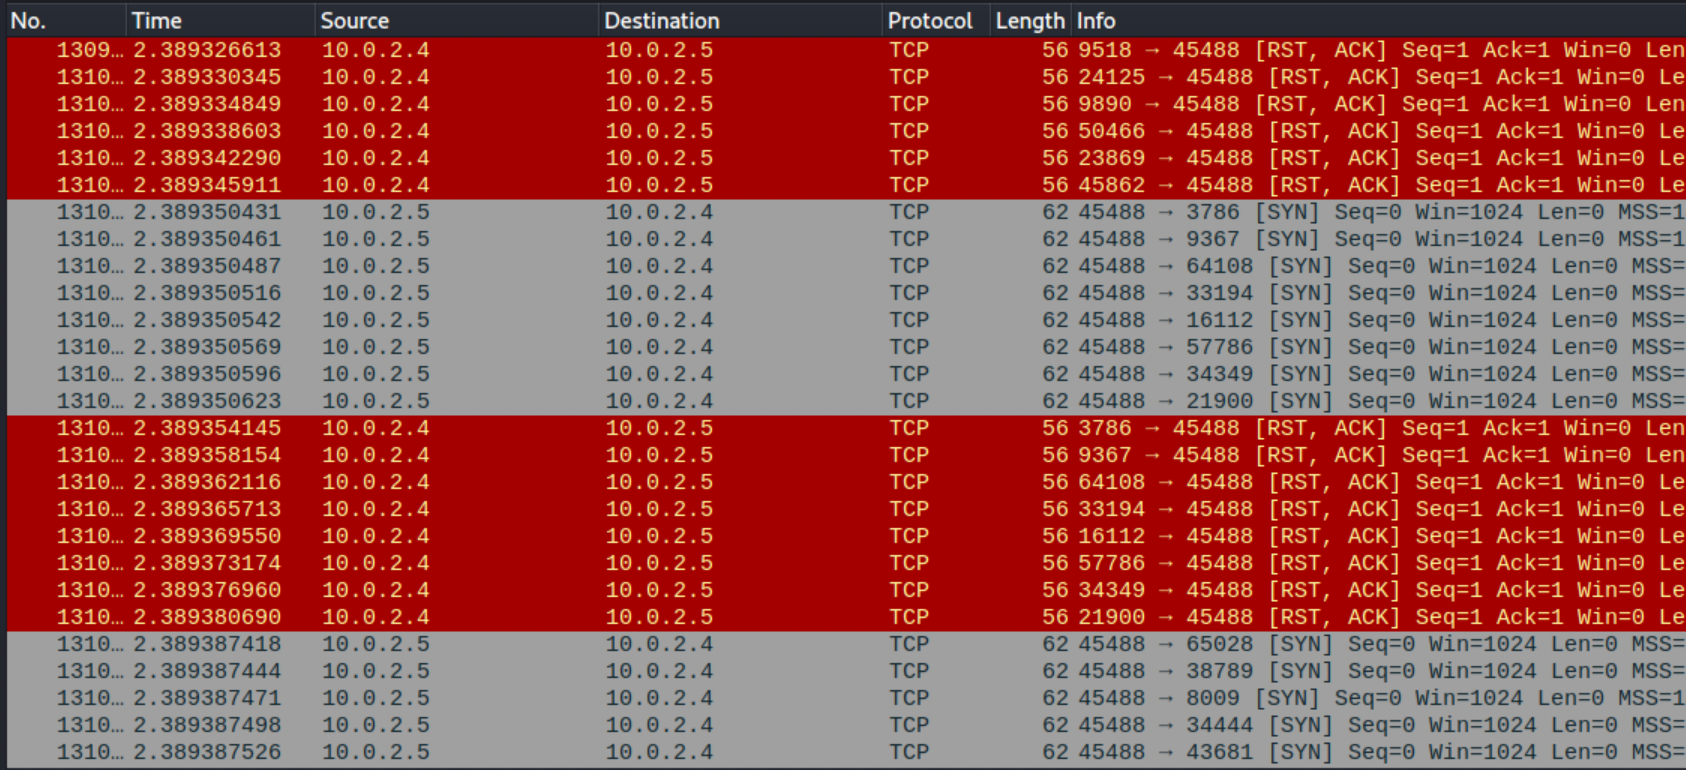
\includegraphics[width=\linewidth]{img/ws_firewall-open.png}
	\caption{Datenverkehr bei offener Firewall}
	\label{fig:ws_firewall_open}
\end{figure}

Im Wireshark-Mitschnitt (Abbildung \ref{fig:ws_firewall_open}) wird der Datenverkehr der Opfermaschine gezeigt. Zu erkennen in grau, sind die eingehenden Anfragen der Angreifermaschine. Hier werden TCP SYN Anfragen an das Opfer geschickt und eine ACK bzw. RST Antwort erwartet. Dies ist die Einleitung einer TCP Verbindung, welche bei diesem Scan nie vollständig durchgeführt wird. Da die Ports der Opfermaschine nicht gefiltert werden, werden die Anfragen verarbeitet und dem Angreifer wird geantwortet. Bei Eingang einer ACK oder RST Nachricht auf der Angreifermaschine wird der Kontakt zum Port abgebrochen und somit keine Verbindung erstellt. Alleine durch das Antworten verrät das Opfer bereits den Status der Ports. Sollte der Angreifer eine ACK Nachricht erhalten, so ist der gefragte Port offen und "hört" auf einkommende Anfragen. Im Falle einer RST Nachricht ist der Port geschlossen.
 Sollte keine Antwort verschickt werden interpretiert NMAP den Port als gefiltert. Ein SYN Scan eignet sich besonders aufgrund der Geschwindigkeit des Scans und der Verlässlichkeit der Ergebnisse.

\subsubsection{nmap 10.0.2.4 -sU -T4}
 Zu prüfen, ob die Verbindung via UDP ebenfalls offen ist, wird als nächster Schritt ein UDP Scan mit NMAP durchgeführt. Wie bei dem vorherigen Scan sind hier ebenfalls die Parameter für die Geschwindigkeit gesetzt. Der -A Parameter wurde gegen -sU ausgetauscht. Der -sU Parameter gibt den Scantyp an. So wird anstatt eines TCP SYN Scans ein UDP Scan durchgeführt. Obwohl TCP den Großteil des Internetverkehrs prägt, ist UDP kein zu vernachlässigendes Protokoll. Bei diesem Scan werden UDP Pakete an die Ports geschickt. NMAP erwartet im Gegenzug ICMP Antworten. Entweder die Opfermaschine schickt eine Nachricht, dass der gewünschte Port nicht erreichbar ist – Port ist geschlossen – oder es wird eine andere Errornachricht verschickt, in welchem Falle der Port als gefiltert gesehen wird. Sollte das Opfer eine UDP Antwort verschicken, so ist der Port offen. Sei es der Fall, dass der Angreifer keine Antwort erhält wird der Port als entweder offen oder gefiltert interpretiert. 
Ein großes Hindernis an UDP Scanning ist der Zeitaufwand, da NMAP bei offenen Ports keine Antwort erhält und daraufhin auf den Timeout warten muss. Auf Grund dessen werden bei diesem Scan nur die wichtigsten 1000 Ports gescannt. Zudem ist die Verbindung via UDP wesentlich unverlässlicher als über TCP, was zu verfälschten Ergebnissen führen kann.

\begin{figure}
	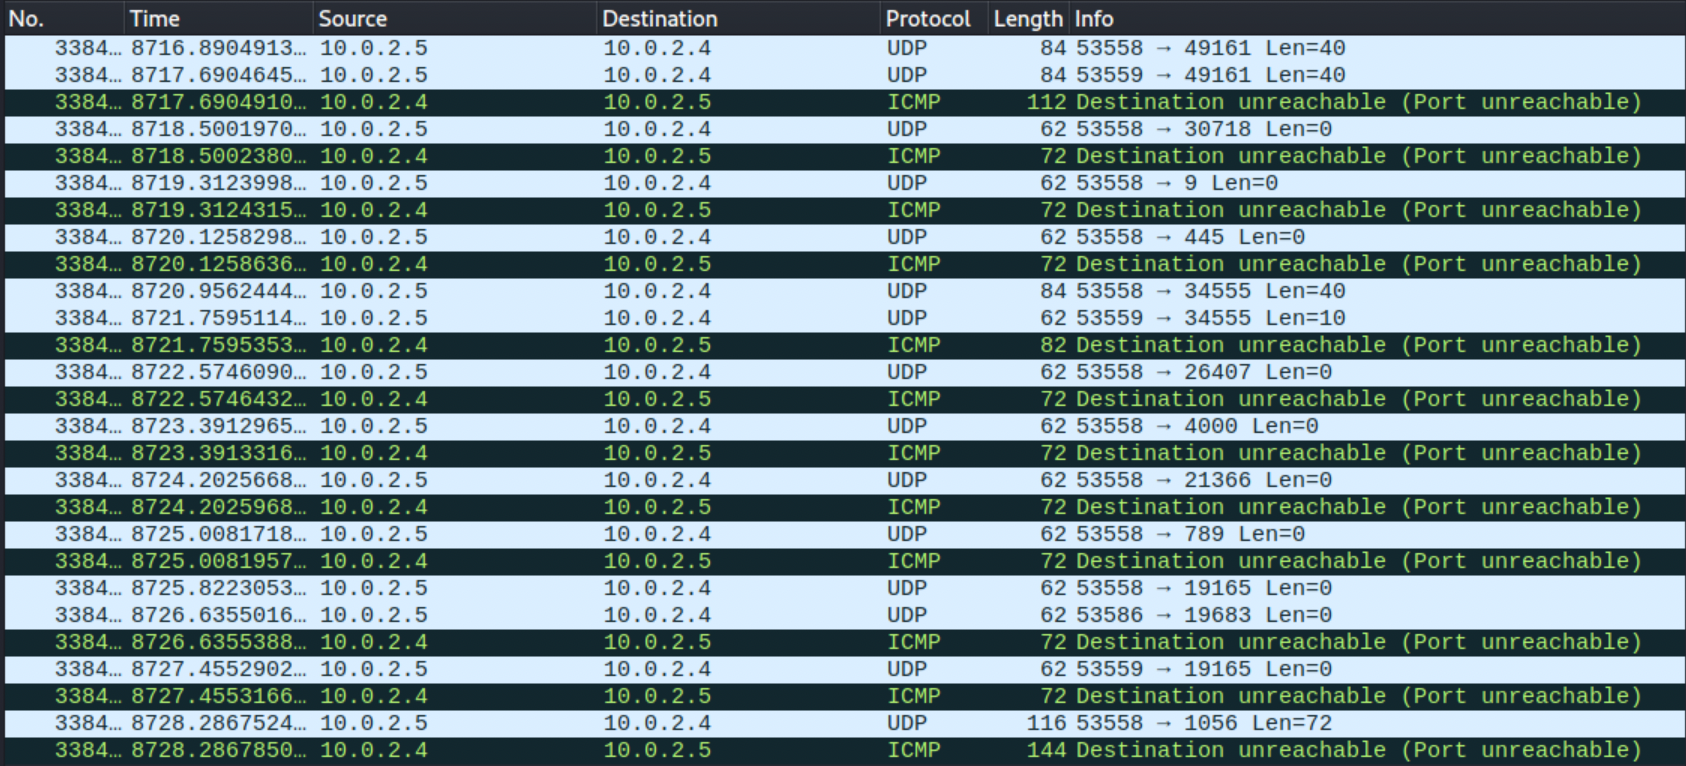
\includegraphics[width=\linewidth]{img/ws_firewall_open_udp.png}
	\caption{Datenverkehr bei offener Firewall – UDP}
	\label{fig:ws_firewall_open_udp}
\end{figure}

Auf der Abbildung \ref{fig:ws_firewall_open_udp} ist zu erkennen, wie der UDP Scan verläuft. Wie bereits beschrieben werden der Opfermaschine UDP Pakete geschickt (zu sehen in Blau). Darauf folgt die Antwort des Opfers – in diesem Fall als ICMP Error – dass der gewünschte Port nicht zu erreichen ist. Aus diesem Grund interpretiert NMAP die Ports der Opfermaschine als geschlossen. \newpage

\lstinputlisting{scripts/scans/nmap_sU_T4}

Am Output des Scans lässt sich erkennen, dass dieser wesentlich länger gebraucht hat als der vorherige TCP Scan. So hat der UDP Scan 18 Minuten gebraucht um die wichtigesten 1000 Ports des Opfers zu scannen. Desweiteren wird berichtet, dass acht Ports offen bzw. gefiltert sind. Da keine Services auf der Opfermaschine laufen oder Firewall-Filter gesetzt sind lässt sich vermuten, dass diese Ports fehlerhaft als offen | gefiltert angezeigt werden. So kann es sein, dass die Opfermaschine nicht schnell genug auf die Anfragen des Angreifers geantwortet haben und somit der Timeout von NMAP erreicht wurde. 

\subsection{Penetrationtest - Outward}
Als nächstes wird getestet, welchen Einfluss die Firewall auf die Funktionalität der Maschine hat. Es werden hierbei zwei Punkte getestet. Zunächst wird mittels wget überprüft, ob das World-Wide-Web erreichbar ist. Daraufhin wird überprüft, ob andere Maschinen im Netzwerk erreicht werden können. 

\subsubsection*{wget https://google.com}

Um zu testen ob das WWW von der Opfermaschine erreichbar ist, wurde mittels des wget Befehls versucht google.com zu erreichen. Das Ziel war es eine index.html von Google zu erhalten und dadurch zu verdeutlichen, dass sowohl HTTPS wie auch DNS auf der Maschine uneingeschränkt funktionieren. Da in dieser Firewall-Konfiguration alle Ports uneingeschränkt sind war davon auszugehen, dass die Maschine ohne Fehler eine index.html erhalten sollte. \\
\begin{figure}
	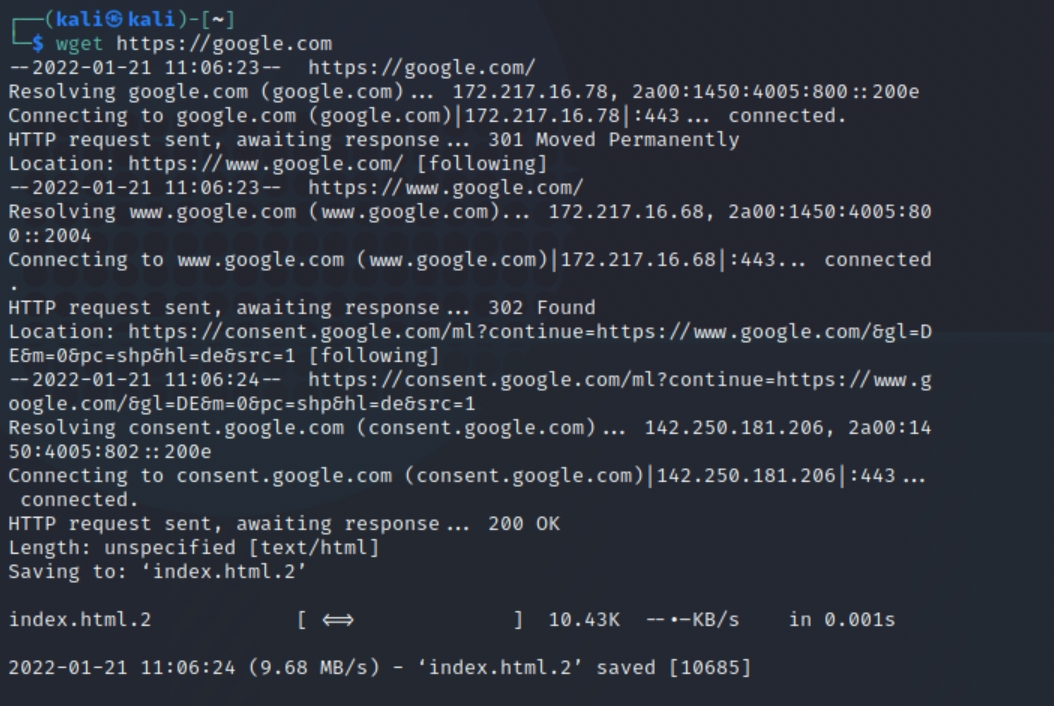
\includegraphics[width=\linewidth]{img/open-in-out-output.png}
	\caption{wget bei offener Firewall-Konfiguration}
	\label{fig:wget_open}
\end{figure}

Wie im Output \ref*{fig:wget_open} zu erkennen, wird auf Anfrage eine index.html von https://google.com erhalten. Demnach lässt sich erkennen, dass sowohl HTTPS wie auch DNS funktionieren. 

\subsubsection*{nc 10.0.2.5 4445}
Als nächstes wurde überprüft, ob eine Verbindung zu einer benachbarten Maschine hergestellt werden kann. Um dies zu testen, wurde über das Tool NetCat versucht eine Verbindung auf dem Port 4445 der Zielmaschine herzustellen. Damit eine Verbindung hergestellt werden kann, wurde auf der Maschine 10.0.2.5 im Terminal der komplementäre Befehl ``nc -lvp 4445 -e /bin/bash' ausgeführt. So weiß die Zielmaschine, auf welchem Port nach Verbindungsanfragen gelauscht werden muss. Zusätzlich erhält der Kommunikationspartner Zugriff auf Konsolenfunktionen der Zielmaschine. So kann nach Verbindungsaufbau kontrolliert werden, dass die Verbindung erstellt wurde. 
\begin{figure}
	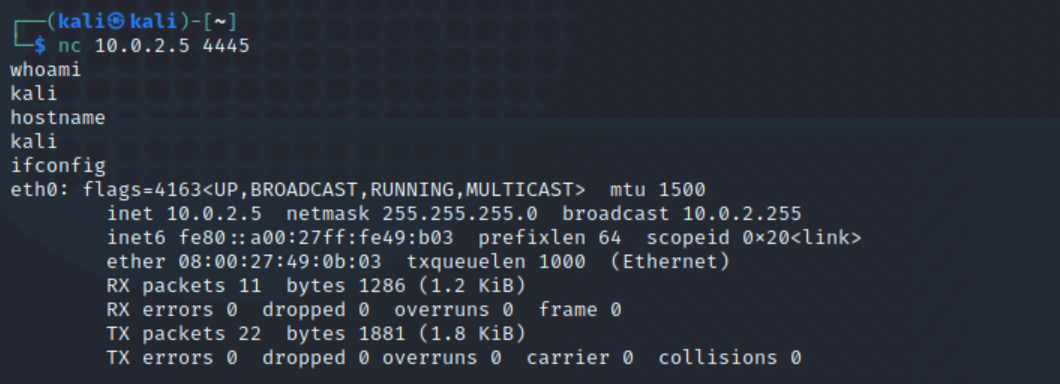
\includegraphics[width=\linewidth]{img/open_nc.png}
	\caption{NetCat-Ergebnis bei offener Konfiguration}
	\label{fig:nc_open}
\end{figure}
\\Im Output \ref{fig:nc_open} lässt sich erkennen, dass die Maschine 10.0.2.4 nun Zugriff auf die Konsole der Maschine 10.0.2.5 besitzt. Durch den Befehl ifconfig, lässt sich dies beweisen. Demnach hat die Verbindung funktioniert, was bei dieser offenen Konfiguration zu erwarten war. 
\section{Geschlossene Konfiguration}
Als nächstes wird eine Konfiguration getestet, in der alle Verbindungen geblockt werden. Zu dieser Konfiguration gehören die Ausnahmen: SSH und localhost. Das Ziel dieses Tests ist es zu prüfen, wie die Opfermaschine von außen angesprochen werden kann – bzw. welche Informationen ein potentieller Angreifer erhalten könnte.
 
\subsection{Script}
Dieses Script besteht aus sechs Teilen: 
\begin{itemize}
	\item Flushing der Regeln
	\item Ausnahmeregelungen
	\item Standardregelungen
	\item Localhost
	\item Bestehende Verbindungen
	\item Logging
\end{itemize}
Zunächst werden alle bestehenden Regeln gelöscht. Dies geschieht wie in dem vorherigen Script mit Hilfe des Flushingbefehls. Darauf folgen die Ausnahmeregelungen. Diese werden hier als nächstes gesetzt, da die Reihenfolge der Regeln bei den IP-Tables durchaus einen Einfluss hat. In diesem Fall wird der Port 22 freigegeben. Sowohl eintreffende wie auch ausgehende Nachrichten dürfen über den Port 22 gehandhabt werden. Dies erlaubt es mit der Virtual Machine eine SSH Verbindung aufzubauen. \\
Um dann die Firewall so einzustellen, dass keine weiteren Verbindungen zugelassen werden, werden nun die Standardregelungen gesetzt. Im Gegenzug zum vorherigen Script werden nun die eingehenden, ausgehenden und weitergeleiteten Verbindungen "gedroppt". So werden alle Pakete die über die betroffenen Ports laufen fallen gelassen und nicht bearbeitet. \\
Damit trotzdessen der localhost weiterhin funktioniert, werden noch einmal Ausnahmen beschrieben.
Zusätzlich werden bestehende Verbindungen weiterhin zugelassen, um keine laufenden Prozesse zu stören. Somit kann gesichert sein, dass plötzliche Änderungen in der Firewall keine Probleme in der Anwendung mitsichziehen. 
Abschließend werden erneut die Loggingbefehle gesetzt.

\newpage

\lstinputlisting[language=bash]{scripts/firewall-closed.sh}

\newpage

\lstinputlisting{scripts/output_firewall-closed}

\subsection{Penetrationtest – Inward}
Nun sind alle Ports der Opfermaschine geblockt bzw. gefiltert. Um zu überprüfen, ob das Script funktioniert hat werden nun eine Reihe an Tests abgeschlossen. Zunächst werden wieder NMAP Scans die Grundlage bilden, von der wichtige Informationen über das Ziel abgeleitet werden können.

\subsubsection{nmap 10.0.2.4 -p- -A -T4}
Es wird nun erneut mittels eines TCP SYN Scans geprüft, welche Ports des Opfers offen sind. Zu Gunsten der Genauigkeit und der Vergleichbarkeit des Scans wurde die Konfiguration der Parameter aus dem Kapitel 2.1.2 übernommen.
Ebenfalls wird erneut der Datenverkehr der Opfermaschine aufgezeichnet. 
\newpage
\lstinputlisting{scripts/scans/nmap_p_A_T4_closed}

An der Ausgabe des Scans lässt sich erkennen, dass trotz der verschärften Regelungen die MAC Adresse sowie der Hersteller des Geräts erkannt wurde. 
Der wichtigste Punkt ist jedoch, dass alle Ports des Opfers nun als gefiltert anstatt als geschlossen erkannt werden. Dies liegt daran, dass keine Antwort auf die SYN Pakete des Angreifers verschickt werden. Wie bereits beschrieben, interpretiert NMAP bei einem TCP SYN Scan das Fehlen einer Antwort als Filterung des angesprochenen Ports. Dies wird anhand der Abbildung \ref{fig:ws_firewall_closed} deutlich. Dort ist zu sehen, wie die Pakete der Angreifermaschine von der Adresse 10.0.2.5 auf der Opfermaschine eintreffen. Jedoch antwortet die Opfermaschine nicht, anders als in Abbildung \ref{fig:ws_firewall_open}.

\begin{figure}
	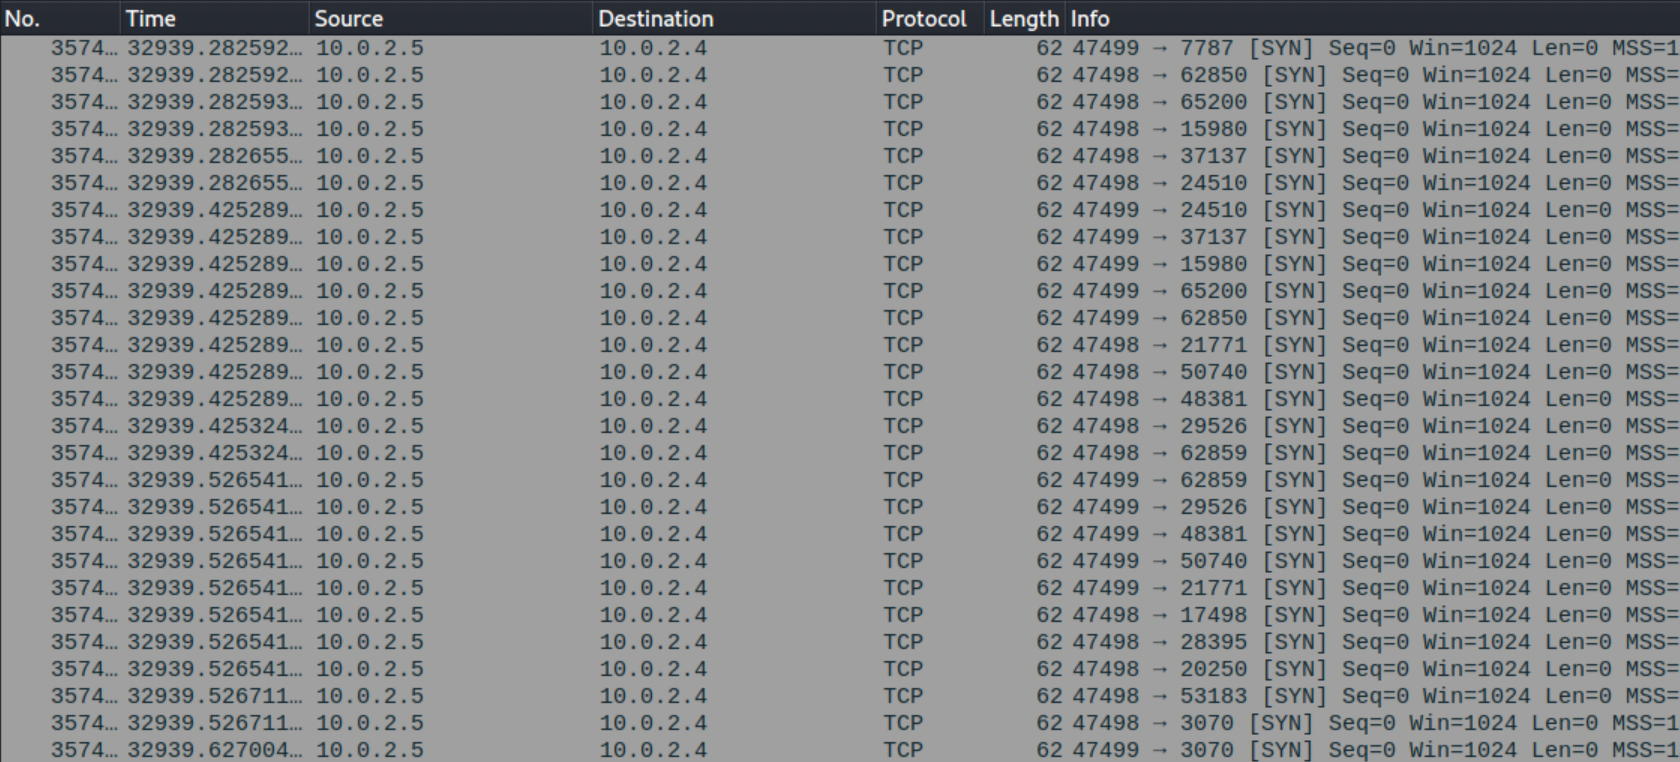
\includegraphics[width=\linewidth]{img/ws_firewall_closed.png}
	\caption{Datenverkehr bei geschlossener Firewall}
	\label{fig:ws_firewall_closed}
\end{figure}

\subsubsection{nmap 10.0.2.4 -sU -T4}
Um zu Prüfen, welchen Einfluss das Script auf UDP Pakete nimmt, wird als nächstes ein UDP Scan durchgeführt. Wie auch beim vorherigen Scan, bleiben die Parameter gleich. Die Erwartung an dieses Scanergebnis ist, dass alle Ports der Opfermaschine als offen | gefiltert angezeigt werden. Zudem wird erwartet, dass dieser Scan wesentlich mehr Zeit in Anspruch nimmt, als der Scan aus dem Kapitel 2.1.2. Diese Erwartungshaltung bildet sich aus der Art und Weise, wie der UDP Scan funktioniert. Da die Ports des Opfers durch das Bash-Script geschlossen sein sollten, sollten keine Antwortpakete an den Angreifer geschickt werden. Somit müsste der Angreifer auf den Timeout von NMAP warten, welcher zur gleichen Zeit die Ports als offen bzw. gefiltert interpretiert.

\begin{figure}
	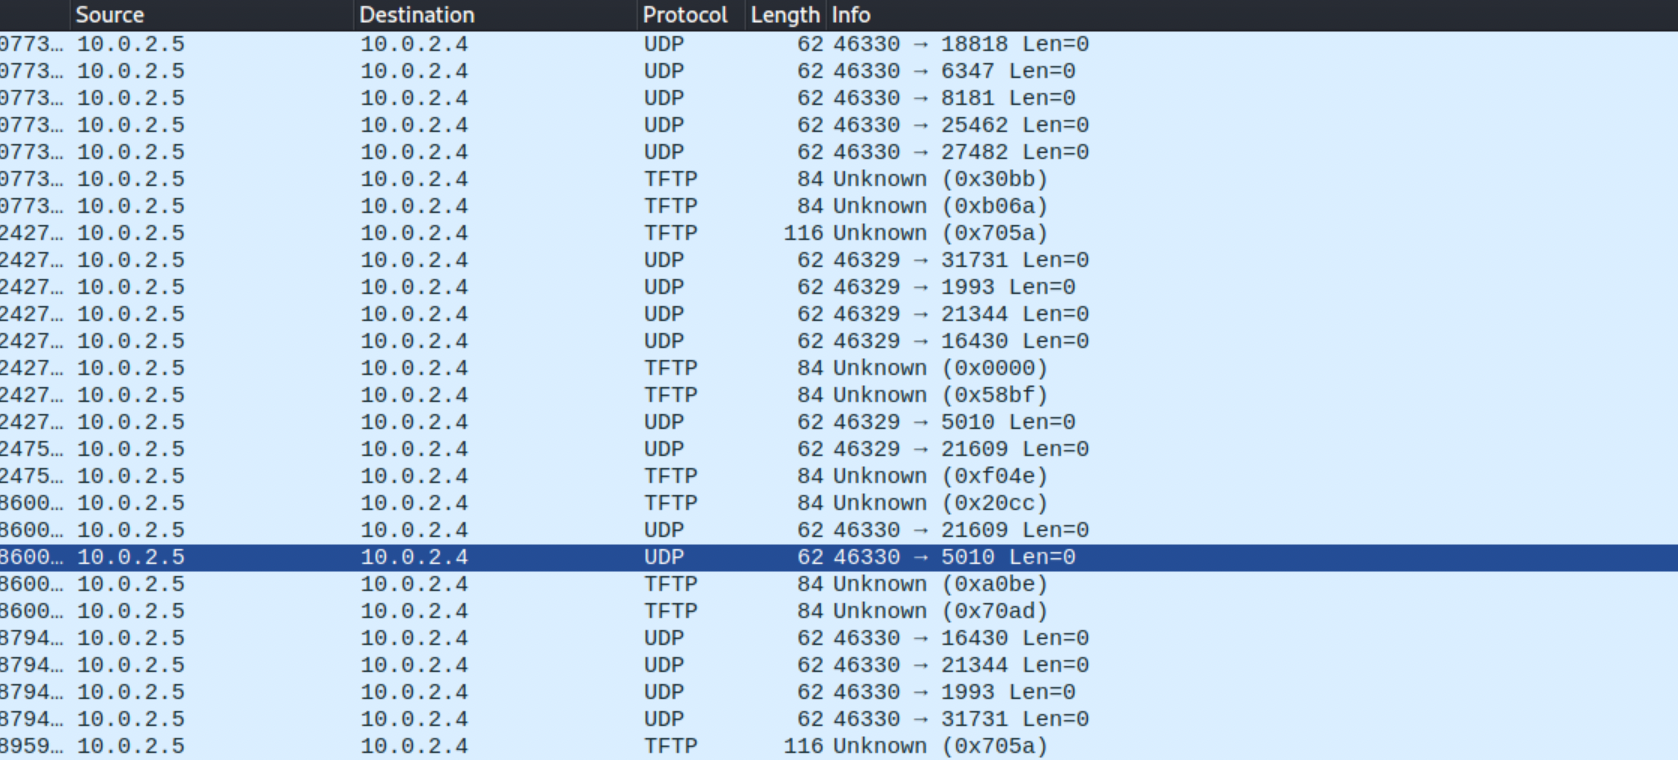
\includegraphics[width=\linewidth]{img/ws_firewall_closed_udp.png}
	\caption{Datenverkehr bei geschlossener Firewall – UDP}
	\label{fig:ws_firewall_closed_udp}
\end{figure}
Output:
\lstinputlisting{scripts/scans/nmap_sU_T4_closed}

Der Output bestätigt die Hypothese. Da der Angreifer keine Antworten erhalten hat, kann keine genaue Aussage über den Status der Ports getroffen werden. 

\subsection{Penetrationtest – Outward}
Wie auch bei der vorherigen Konfiguration, wird gestestet welchen Einfluss die Firewall auf die Funktionstüchtigkeit der Maschine hat. 
Da sowohl eingehende als auch ausgehende Verbindungen von der Firewall geblockt werden, ist es anzunehmen, dass beide Tests fehlschlagen.

\subsubsection*{wget https://google.com}
Zunächst wird erneut getestet, ob das WWW von der Maschine zu erreichen ist. Dafür wird versucht eine index.html von google.com zu erhalten. Da der Port 443 – für https – geblockt ist, ist zu erwarten, dass die Verbindung fehlschlägt. Zudem ist Port 53 – welcher für DNS zuständig ist – ebenfalls geblockt. Was dazu führt, dass der Name google.com keiner IP zugeordnet werden kann. Um zusätzlich zu überprüfen, ob der tatsächliche Server von Google ebenfalls nicht erreichbar ist, wird die IP direkt genutzt. 

\begin{figure}
	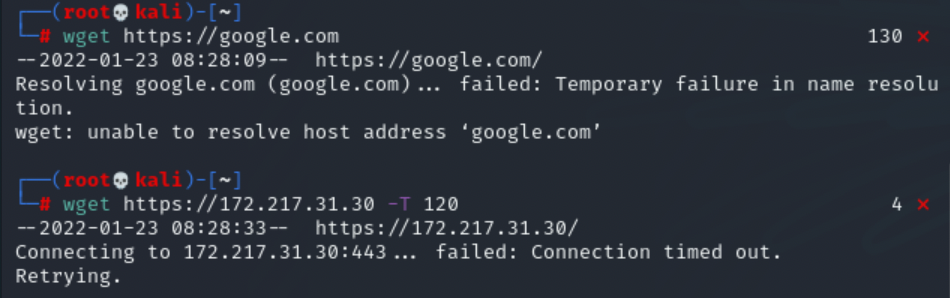
\includegraphics[width=\linewidth]{img/closed-in-out-output.png}
	\caption{Versuch eines Verbindungsaufbaus bei geschlossener Firewall}
	\label{fig:closed_in_out}
\end{figure}

Wie im Output \ref*{fig:closed_in_out} zu erkennen, lässt sich weder über DNS noch über eine direkte IP Adresse eine Verbindung zu google.com aufbauen. Demnach ist es bewiesen, dass die Firewall keine Verbindung ins World Wide Web zulässt.

\subsubsection*{nc 10.0.2.5 4445}

Als nächstes wird getestet, ob die Maschine sich mit einer benachbarten Maschine via NetCat verbinden kann. Da alle Ports geblockt sind, ist zu erwarten, dass keine Verbindung hergestellt werden kann. Das Vorgehen ist das Gleiche, wie im Kapitel 2.1.3.
Zunächst wird auf der Nachbarmaschine – 10.0.2.5 – der Port 4445 mittels NetCat geöffnet und darauf gewartet, dass eine Verbindung hergestellt wird. Daraufhin wird auf der Maschine 10.0.2.4 mittels des NetCat Befehls versucht eine Verbindung aufzubauen. Um zu erkennen, wann eine Verbindung fehlschlägt, wird dem Befehl der Modifier -w angehängt. Dieser erlaubt es eine Sekundenzahl als Timeout anzugeben.
Output:
\lstinputlisting{scripts/nc_closed}
Wie zu erkennen, lässt sich keine Verbindung zu Nachbarmaschine herstellen. Dies war zu erwarten, da alle Ports von der Firewall blockiert werden.

\newpage
\section{Standard Konfiguration}

\lstinputlisting[language=bash]{scripts/firewall-standard.sh}

\subsection{Script}
Das Script zur Erstellung einer Firewall, wie sie möglicherweise in Unternehmen vorkommen könnte, ähnelt dem aus Kapitel 2.2.1 sehr. 
Es besteht aus den gleichen sechs Teilen, obwohl das Logging hier auf Grund der Länge des Scripts vernachlässigt wird.
Zunächst werden alle bestehenden Regeln gelöscht – gefluscht – um die Firewall auf ihre Basiskonfiguration zurückzusetzen. Dies verhindert mögliche Konflikte mit bestehenden Regeln im weiteren Verlauf. \\
Darauf folgend werden alle eingehenden, weiterleitenden und ausgehenden Verbindungen blockiert, bestehende Verbindungen sowie Antworten auf Etablierte werden jedoch weiterhin zugelassen. 
Abschließend werden die Ausnahmeregelungen behandelt, welche den Hauptunterschied zu der vorherigen Konfiguration darstellen. \\
Hier werden die Ports für SSH sowohl eingehend als auch ausgehend zugelassen. Zusätzlich werden die Ports 22, 53, 80 und 443 ausgehend zugelassen, hauptsächlich um Verbindung zum Internet herstellen zu können. 
Zudem sind dem Port 53 UDP Verbindungen gestattet, da das DNS Protokoll hauptsächlich über UDP funktioniert. 

\subsection{Penetrationstest – Inward}
\subsubsection{nmap 10.0.2.4 -p- -A -T4}
Wie auch bei den vorherigen Konfigurationen, wird hier ebenfalls zunächst ein TCP SYN Scan durchgeführt. Da in dieser Firewall-Konfiguration keine fundamentalen Veränderungen durchgeführt wurden, werden den Vorgängern ähnliche Ergebnisse erwartet. Es sollte der Angreifermaschine nur ein Port ersichtlich sein, da alle Anderen nur von innen nach außen funktionieren. \\
Output:
\begin{figure}
	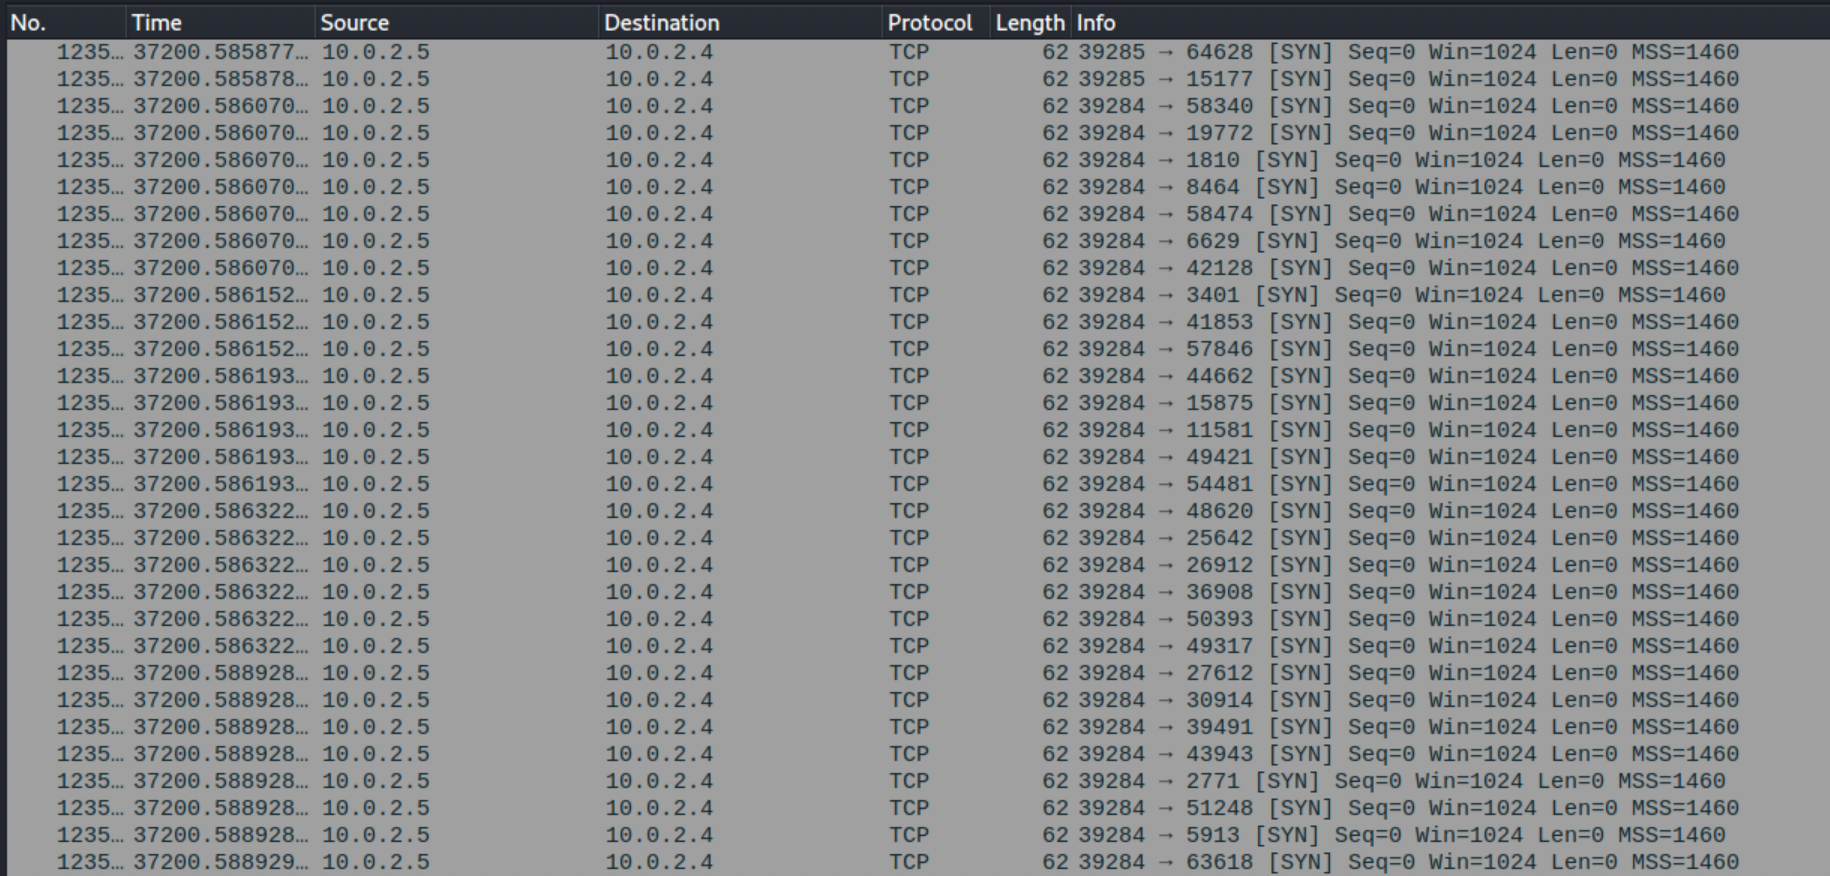
\includegraphics[width=\linewidth]{img/ws_firewall_standard.png}
	\caption{Datenverkehr der Opfermaschine}
	\label{fig:ws_firewall_standard}
\end{figure}

\lstinputlisting{scripts/scans/nmap_p_A_T4_standard}

Der Output dieses Scans ist identisch mit dem aus Kapitel 2.2.2, mit der Ausnahme des Ports 22. Ein maßgeblicher Unterschied wird sich erst bei einem ausgehenden Test erkennen lassen.

\begin{figure}
	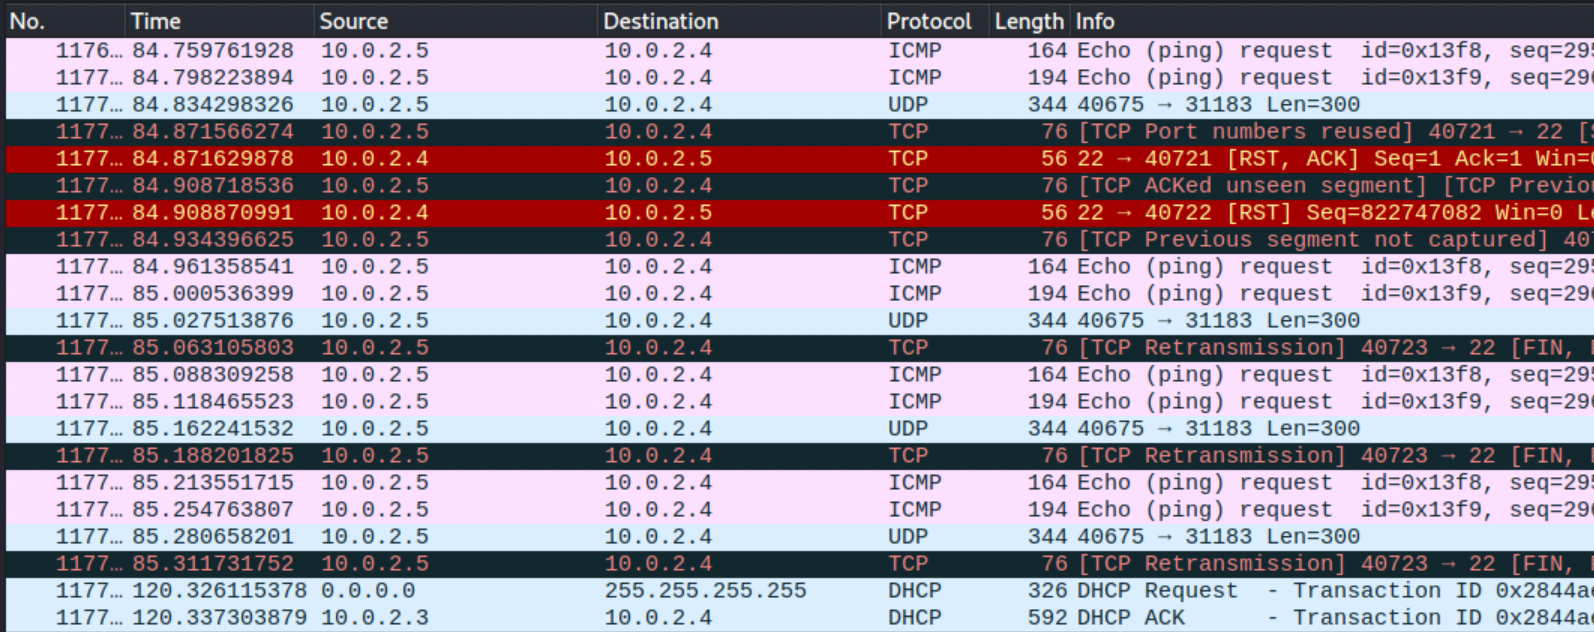
\includegraphics[width=\linewidth]{img/ws_firewall_standard_2.png}
	\caption{Fort.: Datenverkehr der Opfermaschine}
	\label{fig:ws_firewall_standard_2}
\end{figure}

\subsubsection{nmap 10.0.2.4 -sU -T4}
Im Script wurde der Port 53, welcher für das DNS Protokoll verwendet wird, für ausgehende UDP Pakete geöffnet. Diese Ausnahmeregelung ist die Einzige, die UDP betrifft. Da die Ausnahme nur für ausgehende Pakete gilt, ist es zu erwarten, dass ähnlich wie in Kapitel 2.2.2 alle Ports als ``open | filtered`` gezeigt werden. \\
Output: 

\lstinputlisting{scripts/scans/nmap_sU_T4_standard}
\begin{figure}
	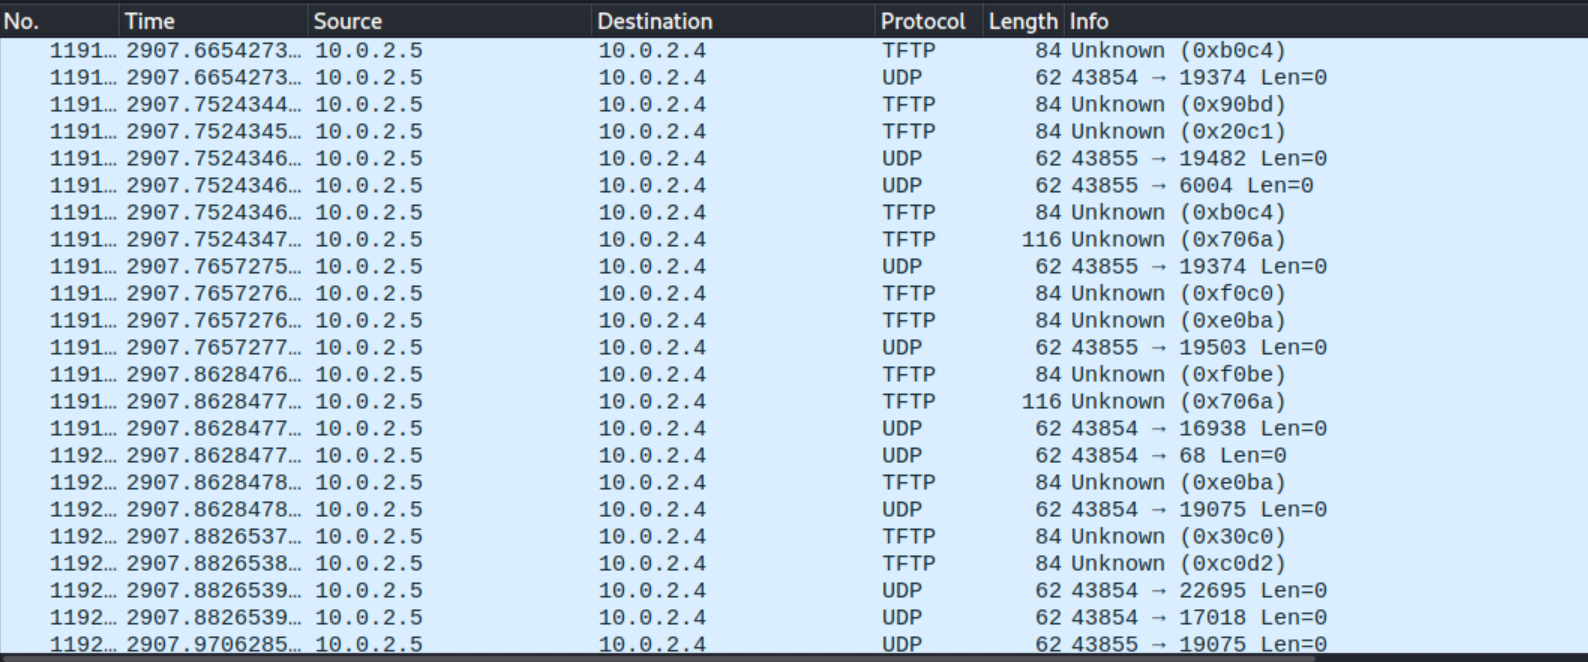
\includegraphics[width=\linewidth]{img/ws_firewall_standard_udp.png}
	\caption{Datenverkehr der Opfermaschine – UDP}
	\label{fig:ws_firewall_standard_udp}
\end{figure}
\subsection{Penetrationtest – Outward}

Abschließend wird auch bei dieser Firewall-Konfiguration überprüft, welchen Einfluss die Firewall auf die ausgehenden Verbindungen der Maschine besitzt. Das Verfahren ist gleich dem der zwei Vorgängern. 

\subsubsection*{wget https://google.com}
Zunächst soll getestet werden, ob google.com erreichbar ist. Die Ports für http und https sind beide in die ausgehende Richtung freigegeben, demnach sollte es zu erwarten sein, dass eine Verbindung zum WWW hergestellt werden kann. Zusätzlich wurde der Port 53 für DNS freigegeben. So sollte es möglich sein über die Domain google.com eine Verbindung aufzubauen. 
\begin{figure}
	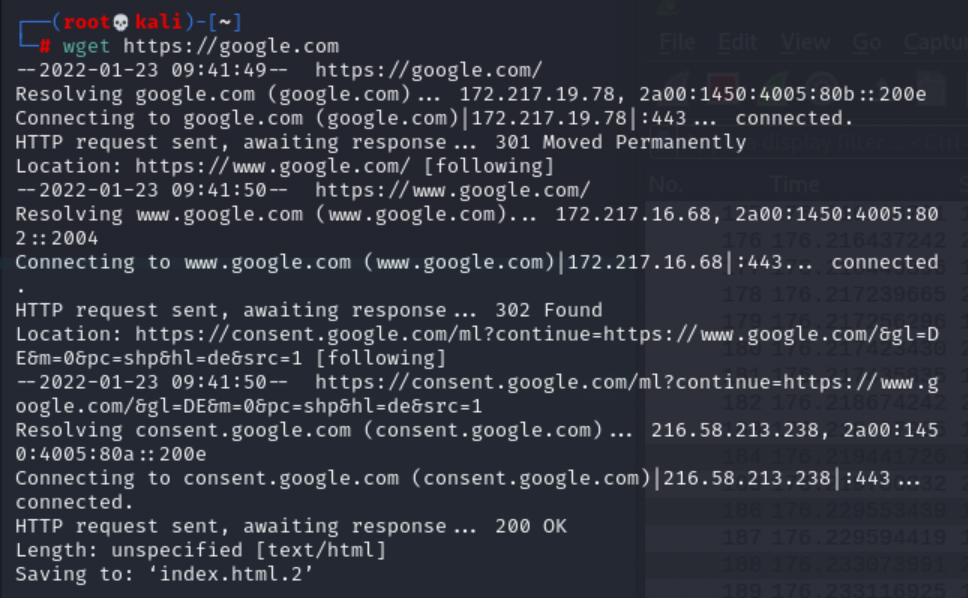
\includegraphics[width=\linewidth]{img/standard_in_out_output.png}
	\caption{Erfolgreicher Verbindungsaufbau zum WWW bei Standardfirewall}
	\label{fig:standard_in_out}
\end{figure}

Wie im Output \ref{fig:standard_in_out} zu erkennen, lässt sich sowohl die Domain google.com auflösen, wie auch eine Verbindung zu der Gleichen herstellen. Dies lässt darauf schließen dass die freigegeben Ports ordnungsgemäß funktionieren, obwohl sie nur in eine "Richtung" freigegeben sind. Dies funktioniert, da established connections – also etablierte Verbindungen – freigegeben sind. Das bedeutet dass Antworten auf die Anfragen der Maschine durch die Firewall kommen aber fremde Anfragen nicht. Dies hilft dabei ungewünschte Verbindungen vorzubeugen.

\subsubsection*{nc 10.0.2.5 4445}
Abschließend soll nun getestet werden, ob die Maschine eine Verbindung zu ihrem Nachbarn über arbiträre Ports aufbauen kann. Dafür wird erneut mittels des NetCat Befehls versucht eine Verbindung zur Maschine auf 10.0.2.5 aufzubauen. 
Der Befehl auf dieser Nachbarmaschine ist gleich dem der anderen Tests aus Kapiteln 2.1.3 und 2.2.3. Genau so ist der Befehl auf der Maschine 10.0.2.4 gleich. Da bis auf ein paar Ausnahmen alle Ports weiterhin von der Firewall geblockt werden, ist es anzunehmen das dieser Verbindungsaufbau fehlschlagen wird. Es wird wieder ein Timeout von 60 Sekunden eingestellt. 

\lstinputlisting{scripts/nc_closed}

Wie zu erkennen ist es erneut fehlgeschlagen eine Verbindung zur Nachbarmaschine aufzubauen. 

\chapter{Projektphase 2 – Webserver}
Die Phase Webserver soll demonstrieren, für welche typischen Angriffsmethoden Webseiten anfällig sind. Dabei werden im Rahmen der Demonstration zwei Angriffe durchgeführt – eine \ac{XSS} Attacke und eine SQL Injection. 
\section{Setup}
\subsection{Datenbank}
Für das Projekt wurde PostgreSQL (auch einfach als Postgres bezeichnet) als Datenbank gewählt. So wurde über Docker eine Container-Instanz einer Postgres Datenbank gestartet, die auf einem Port auf der Hostmaschine auf Nachrichten wartet und über die Adresse localhost:5432 erreichbar ist. \\
Die Datenbank enthält ein Schema "blog", welches die beiden Tabellen – User und Post – beinhaltet. Diese beiden Tabellen besitzen jeweils eine inkrementierende ID als Primärschlüssel. 

\begin{figure}
    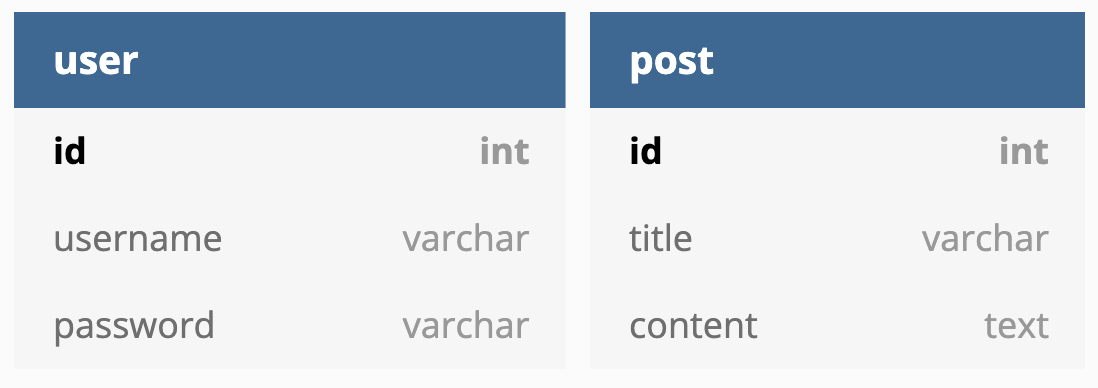
\includegraphics[width=\linewidth]{img/database.png}
    \caption{Database Setup}
    \label{fig:database}
\end{figure}

Die Tabelle User enthält dabei zusätzlich den Benutzernamen und das Passwort des Nutzers – wobei beide bewusst im Klartext gespeichert werden. 
Die Tabelle Post enthält neben der ID noch die Attribute Title und Content, welche bei der Ausgabe der Posts angezeigt werden. 
Als Vorbereitung für die Demonstration beider Attacken wurden bereits Beispiel-Posts und User angelegt, um ein anschaulicheres Ergebnis zu erhalten.
\pagebreak
\subsection{API}

\begin{figure}
    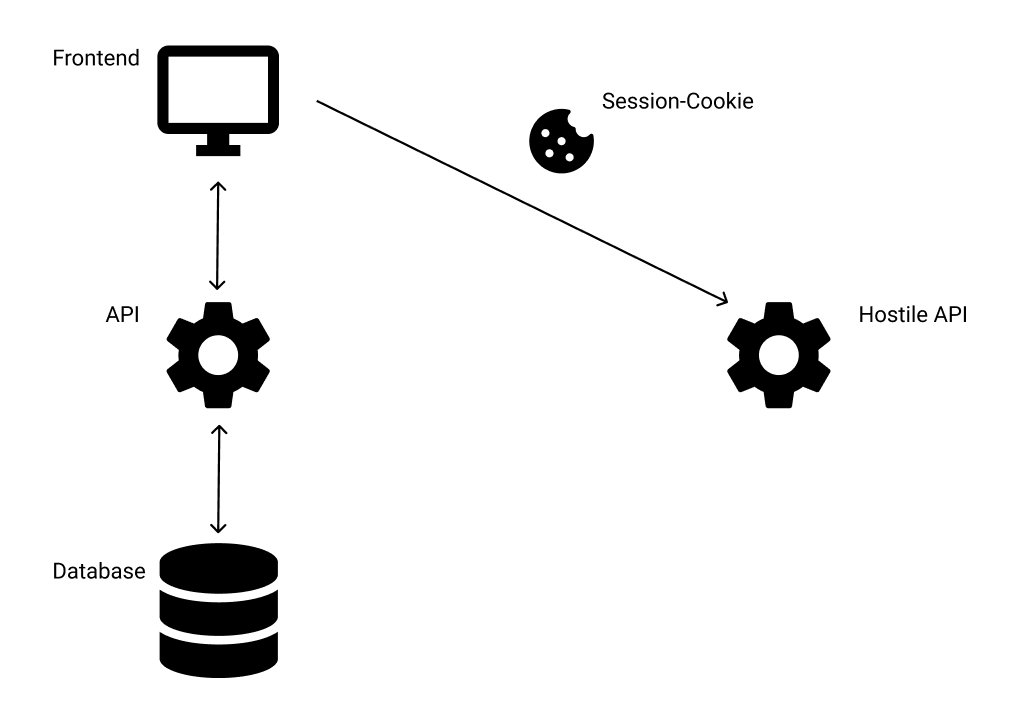
\includegraphics[width=\linewidth]{img/phase2.png}
    \caption{API Setup}
    \label{fig:api}
\end{figure}
Zur Demonstration der beiden Attacken werden zwei APIs genutzt. Beide werden mit Hilfe des Express.js Frameworks implementiert. \\
Die erste – und umfangreichere – API stellt die Schnittstelle zur Datenbank der Blog-Applikation dar. Hier werden die typischen CRUD Operationen durchgeführt und ans Frontend angebunden. Zudem wird die Session-Erstellung hier geregelt.\\
Zu Demonstrationszwecken wurden bewusst Sicherheitsfunktionen in dieser API umgangen. Es wurde zum Beispiel darauf verzichtet, das HTTPOnly Attribut des Cookies zu setzen, was den Zugriff auf den Cookie aus einem Skript heraus verhindern würde. Zudem wird der Cookie im Klartext verschickt, anstatt verschlüsselt zu werden, was ebenfalls die potentielle Sicherheit der Demonstrationsapplikation untergräbt.\\
Die andere API – im Weiteren als bösartige API bezeichnet – stellt den Angreifer dar. Sie verfügt nur über eine einzige Methode, über welche der Session-Cookie des Opfers abgefangen wird. 
\subsection{Frontend}
Das Frontend bildet einen Weblog ab, welcher das Posten von Textbeiträgen ermöglicht. Im Eingabeformular werden vom Besucher Titel und Inhalt eingetragen, bestätigt ("Submit") und über die API an das Backend übermittelt, wo sie in der Datenbank gespeichert werden.\\
Das Frontend wurde mit Vue.js entwickelt und bietet aus diesem Grund einige vordefinierte und standardmäßig aktivierte Sicherheitsfunktionen, die eine \ac{XSS}
 Attacke verhindern sollen. 
\begin{figure}
    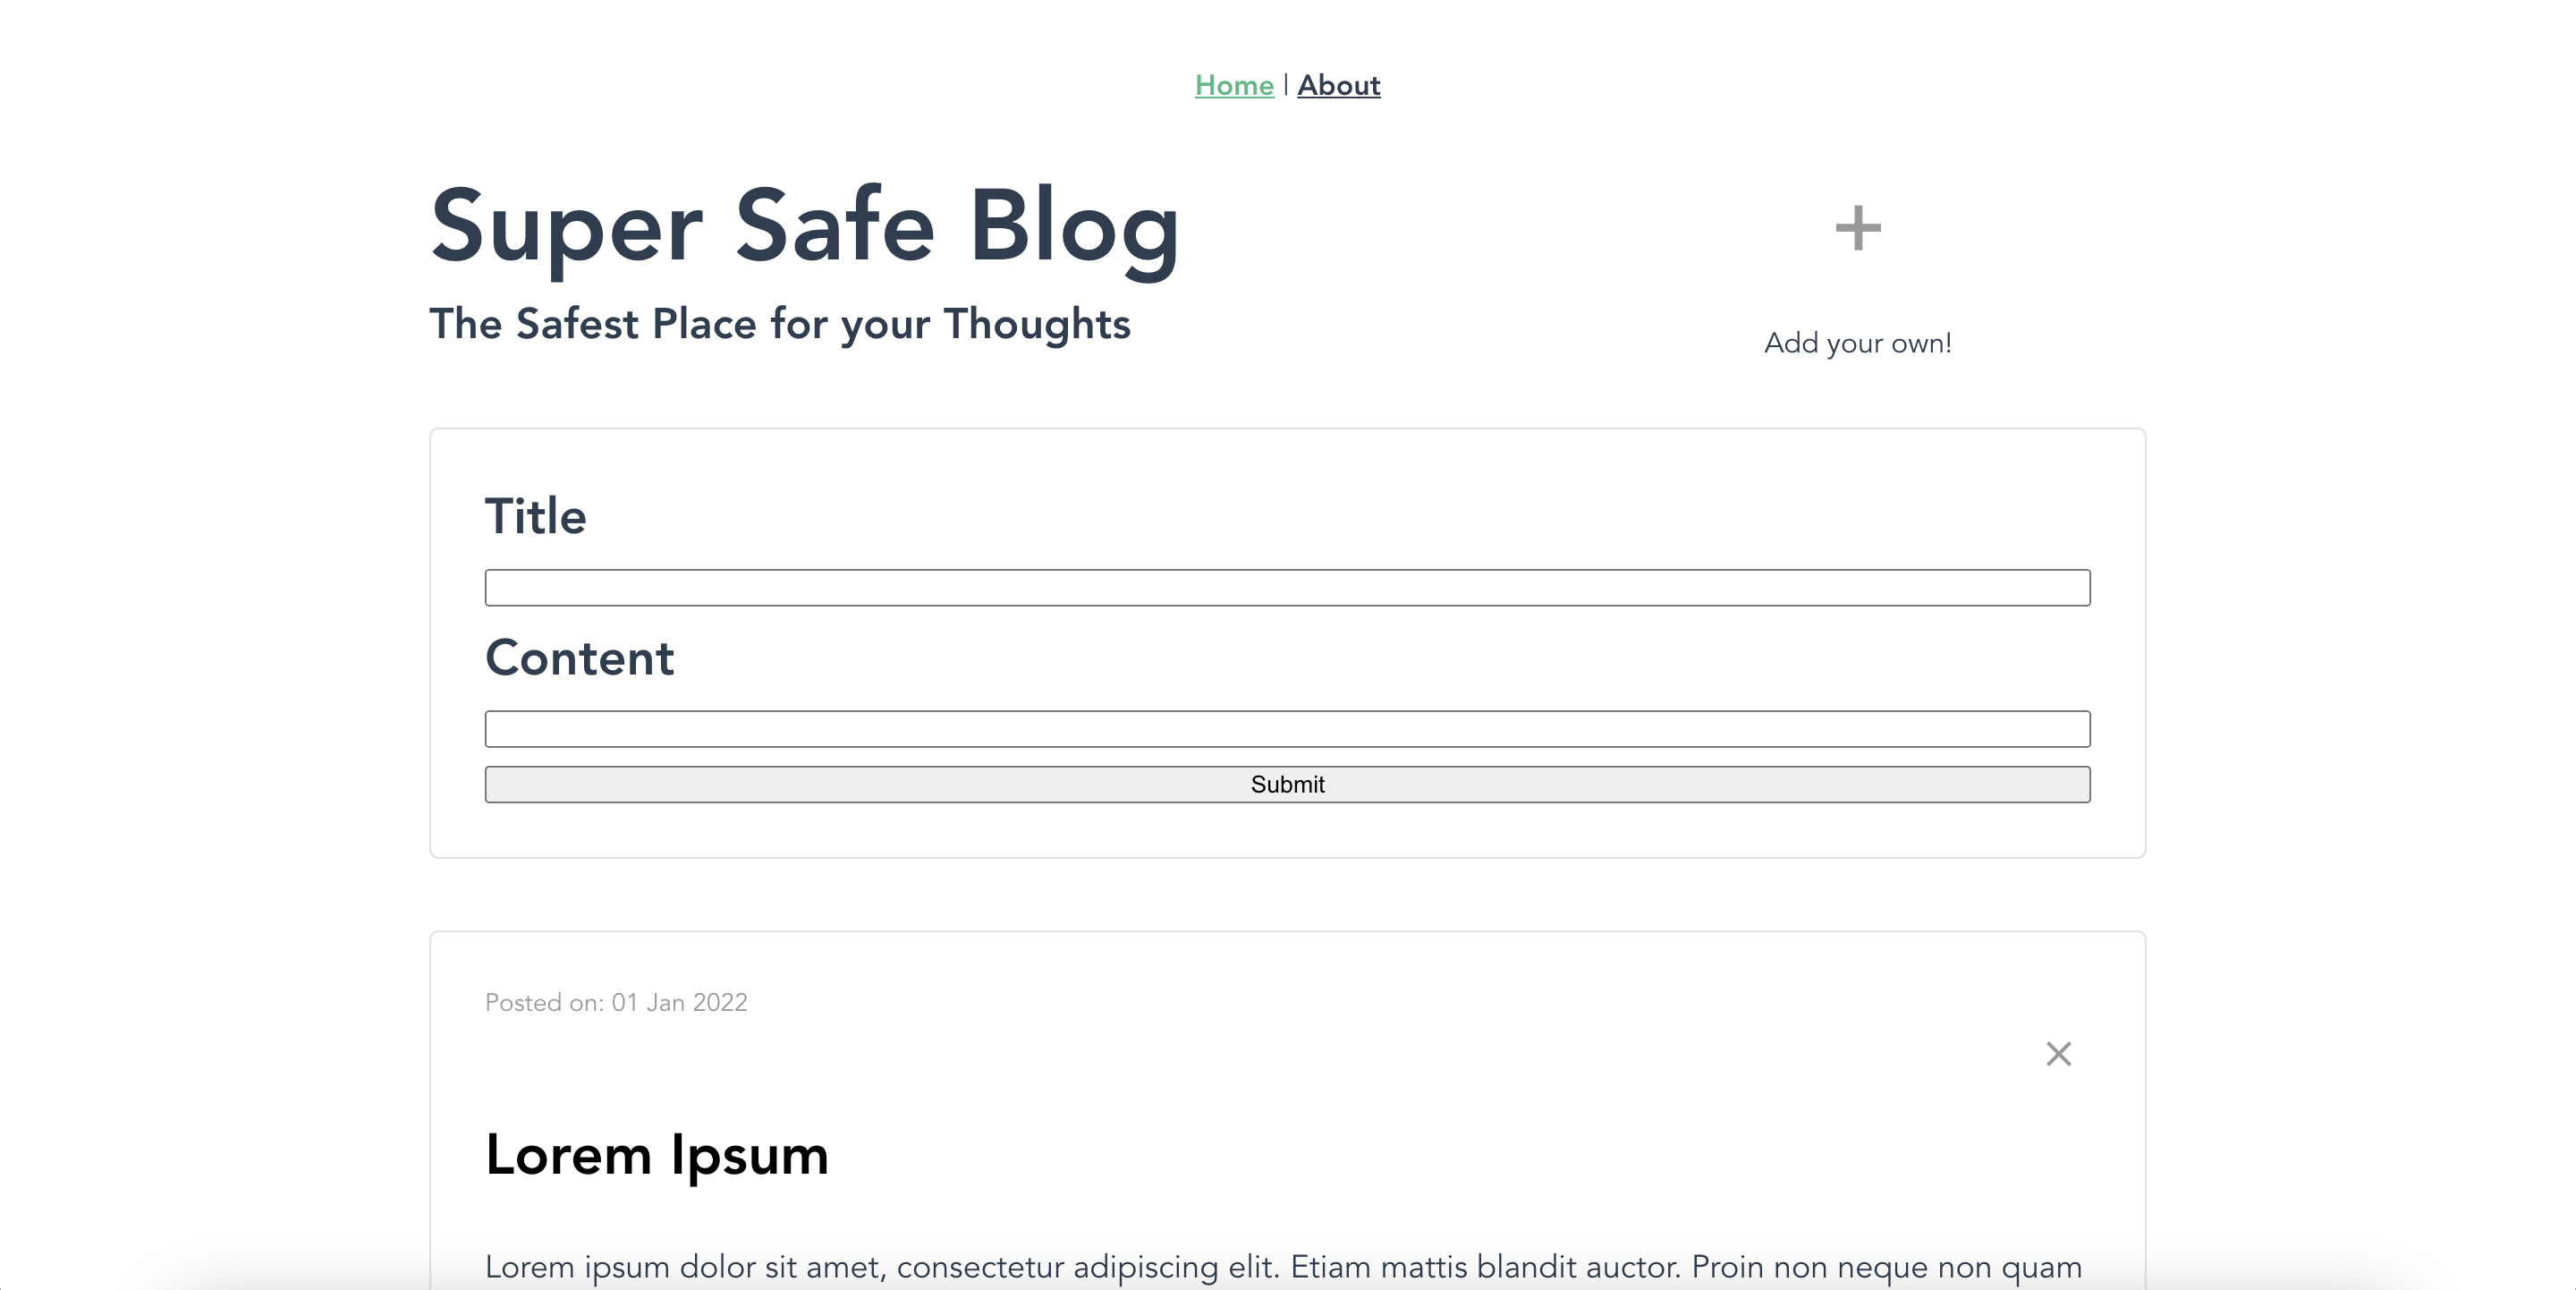
\includegraphics[width=\linewidth]{img/blog.png}
    \caption{Blog-Frontend}
    \label{fig:frontend}
\end{figure}
Um diese Sicherheitsmechanismen zu umgehen, werden die Inhalte aus der Datenbank mit Hilfe des v-HTML Attributs in das Frontend eingebunden, anstatt mit der üblichen ``Mustache`` Notation oder dem v-text Attribut. Diese füllen das innerText Attribut der DOM-Node mit dem gewünschten Inhalt, werden jedoch automatisch ``escaped'', was im Sinne der Sicherheit ist, jedoch gerade die hier beabsichtigte Simulation eines XSS-Angriffes verhindert. . 

\section{Cross-Site-Scripting}

Unter dem Begriff \ac{XSS} versteht man einen Typ der Injektionsattacken, bei dem schadhafter Code – oft in Form eines browserseitigen Scripts – bei einem Endnutzer ausgeführt wird. Diese werden unter anderem durch mangelhafte bzw. fehlende Überprüfung von Nutzereingaben ermöglicht. \\
Um dieses zu demonstrieren, wurde bei diesem Projekt bewusst darauf verzichtet, Nutzereingaben zu überprüfen. 
Das Ziel der Demonstration ist es den Session-Cookie zu stehlen. Um dies zu erreichen wird ein neuer Blog-Post erstellt, bei dem an Stelle eines ``einfachen'' Textes als Inhalt ein schadhaftes HTML <img> Element eingegeben wird. Da es sich bei diesem Element letztlich nur um Text handelt und die Eingabe nicht überprüft wird, wird der Wert in der Datenbank gespeichert. Beim erneuten Aufrufen der Seite versucht der Browser, das <img> Element wie jedes andere auch als Bild zu rendern, erhält jedoch nur einen Fehler, da die im src-Attribut als Bildquelle angegebene URL bewusst fehlerhaft ist. \\
Nun ist es möglich mittels des HTML Attributs ``onerror'' der Applikation vorzuschreiben, wie mit dem Fehler umzugehen ist. Dies wird mittels validem JavaScript Code geschafft. 

    \lstinputlisting{scripts/xss}

Im onerror Attribut wird nun zunächst der Session-Cookie in der Variable cookies gespeichert und dann an die an die Adresse des Angreifers über die bösartige API übermittelt. Sobald der Vorgang abgeschlossen ist wird im Browser-Fenster des Opfers über ein Alert angezeigt, dass das Script funktioniert hat. Abschließend ist der Session-Cookie auf der Console des bösartigen Servers zu finden.

Der Angreifer wäre nun in der Lage diesen Session-Cookie zu nutzen, um sich auf der betroffenen Webseite als ``Opfer'' auszugeben. Demnach könnte der Angreifer die digitale Identität des Opfers stehlen. 
Somit hätte er Zugriff auf die Kontoeinstellungen des Opfers oder er könnte Bestellungen im Namen und mit den Zahlungsmitteln des Opfers tätigen. \\
Große Online-Shops, wie zum Beispiel Amazon, versuchen solche (und ähnliche) Probleme zu verhindern, indem sie vor der Transaktion eine erneute Authentifizierung fordern. So braucht der Angreifer zusätzlich noch Passwort und Benutzername des Opfers, wenn nicht sogar MFA eingerichtet ist.

\section{SQL Injection}
Als zweite Demonstration wird eine SQL Injection durchgeführt. SQL Injections sind eine Art der Injektionsattacken, bei der durch Nutzereingaben valide SQL Queries in die betroffene Applikation injiziert werden. Die OWASP Foundation schreibt dazu: 
\begin{quote}
    A SQL injection attack consists of insertion or “injection” of a SQL query via the input data from the client to the application. A successful SQL injection exploit can read sensitive data from the database, modify database data (Insert/Update/Delete), execute administration operations on the database (such as shutdown the DBMS), recover the content of a given file present on the DBMS file system and in some cases issue commands to the operating system. \cite{abc}
\end{quote}

Das Ziel dieser Demonstration ist es, durch die Eingabe einer bestimmten Zeichenkette einen fremden Post gezielt zu löschen. Dafür wird ein neuer Post eröffnet, bei welchem der Titel frei gewählt, im Content jedoch der folgende String eingegeben wird: 

\lstinputlisting{scripts/injection.sql}

Der String funktioniert, indem zunächst die ursprüngliche Query escaped wird und darauf folgend eine weitere bösartige Query. 
Standardmäßig nutzt die API eine Query, welche mit der Schreibweise ``VALUES ('\$\{Title\}', '\$\{Content\}')' endet, um neue Posts in der Datenbank anzulegen. Wenn nun in der Variable Content die Zeichen '); in Reihenfolge auftreten, werden diese von der Datenbank als Abschluss der Query interpretiert. Daraufhin wird dann eine weitere bösartige Query angehängt, welche von der Datenbank aufgegriffen und verarbeitet wird. Diese Query gibt der Datenbank die Anweisung alle Posts zu löschen, bei denen der Titel ``test'' lautet. 
In einer Produktionsumgebung, wie zum Beispiel die eines Online-Shops, könnte ein derartiger unauthorisierter Eingriff erhebliche Folgen mitsichziehen. So könnte ein bösartiger Akteur sämtliche Inhalte der Datenbank löschen oder publizieren. 
Ähnlich wie die \ac{XSS} Attacken können SQL Injections verhindert werden, indem Nutzereingaben escaped werden.


% Fazit und Ausblick
%% !TEX root =  master.tex
\chapter{Zusammenfassung}

\nocite{*}


\section{Fazit}

Das Bewusstsein für und die Auseinandersetzung mit dem Thema Work-Life-Balance ist mit gut 20 Jahren noch sehr jung. Dennoch hat es sich in dieser kurzen Zeit mit Nachdruck im gesellschaftlichen Diskurs und in der individuellen Priorisierung festgesetzt. Die durchweg positiven Auswirkungen von Work-Life-Balance-Maßnahmen lassen sich betriebswirtschaftlich, gesamtgesellschaftlich (volkswirtschaftlich) und auf der Ebene des Individuums nachweisen. Unternehmen stehen eine ganze Reihe von bewährten Maßnahmen zur Erhöhung der Vereinbarkeit von Privatleben und Erwerbsleben zur Verfügung, die sie nutzen müssen, wenn sie nicht abgehängt werden wollen.

\section{Ausblick}

Weltweit betrachtet gibt es noch erheblichen Nachholbedarf zum Thema Work-Life-Balance. Die Ausprägung hängt jedoch mit dem Entwicklungsstand der jeweiligen Gesellschaften und Ökonomien zusammen und kann sich nur im Rahmen der Veränderungen mit entwickeln.
Auch in Deutschland besteht Potential für weitere Verbesserungen, die durch gesetzliche und gesellschaftliche Rahmenbedingungen gesteuert und gestaltet werden können. Im Zuge der Corona-Pandemie wurde aufgezeigt, mit welchem Tempo sich manche Rahmenbedingungen ändern lassen, hier ist insbesondere auf die Ermöglichung von Remote-Arbeit hinzuweisen. Andere Bestrebungen hingegen, die etwa aus der New-Work-Bewegung kommen, oder auf weitere Reduktionen der Wochenarbeitszeit hinwirken oder gar die Einführung eines bedingungslosen Grundeinkommens fordern, werden voraussichtlich noch mehrere Generationen auf eine Realisierung warten müssen.



%%%%%%%%%%%%%%%%%%%%%%%%%%%%%%%%%%%

\initializeAppendix

%%%%%%%%%%%%%%%%%%%%%%%%%%%%%%%%%%%
% ANHÄNGE
%
% @stud: einzelne Anhänge bearbeiten und eigene Anhänge hier einfügen 
%
%\input{appendix1}
%\input{appendix2}
%%%%%%%%%%%%%%%%%%%%%%%%%%%%%%%%%%%

%%%%%%%%%%%%%%%%%%%%%%%%%%%%%%%%%%%
% LITERATURVERZEICHNIS
% 
% @stud: Literaturverzeichnis in Datei bibliography.bib anpassen 
%
\initializeBibliography
%%%%%%%%%%%%%%%%%%%%%%%%%%%%%%%%%%%

\addcontentsline{toc}{chapter}{Index}
\printindex

\end{document}
